\iffalse
\documentclass[12pt]{article}
\usepackage{graphicx}
%\documentclass[journal,12pt,twocolumn]{IEEEtran}
\usepackage[none]{hyphenat}
\usepackage{graphicx}
\usepackage{listings}
\usepackage[english]{babel}
\usepackage{graphicx}
\usepackage{caption} 
\usepackage{hyperref}
\usepackage{booktabs}
\usepackage{commath}
\usepackage{gensymb}
\usepackage{array}
\usepackage{amsmath}   % for having text in math mode
\usepackage{mathtools}
\usepackage{listings}
\let\vec\mathbf
\lstset{
  frame=single,
  breaklines=true
}
  
%Following 2 lines were added to remove the blank page at the beginning
\usepackage{atbegshi}% http://ctan.org/pkg/atbegshi
\AtBeginDocument{\AtBeginShipoutNext{\AtBeginShipoutDiscard}}
%
%New macro definitions
\newcommand{\mydet}[1]{\ensuremath{\begin{vmatrix}#1\end{vmatrix}}}
\providecommand{\brak}[1]{\ensuremath{\left(#1\right)}}
\providecommand{\norm}[1]{\left\lVert#1\right\rVert}
\newcommand{\solution}{\noindent \textbf{Solution: }}
\newcommand{\myvec}[1]{\ensuremath{\begin{pmatrix}#1\end{pmatrix}}}
\let\vec\mathbf
\begin{document}
\begin{center}
\title{\textbf{LINES}}
\date{\vspace{-5ex}} %Not to print date automatically
\maketitle
\end{center}
\setcounter{page}{1}
\section*{CHAPTER 11 - STRAIGHT LINES}
\section*{Excercise 10.3}
\solution 
\begin{enumerate}
\section{Solution}
		\fi
		Let
\begin{align}
 \vec{P}=\myvec{
-1\\
3
}
\end{align}
The line parameters are
\begin{align}
\vec{n}=\myvec{
3\\
-4
}, c=16
\end{align}
The desired foot of the perpendicular is then given by 
\begin{align}
\myvec{4&3\\3&-4}\vec{A}&=\myvec{\myvec{4&3}\myvec{-1\\3}\\16}\\
&=\myvec{5\\16}  
\end{align}
The augmented matrix for the above system is
\begin{align}
  \myvec{
   4 &  3  & 5\\
   3 & -4  & 16} 
  \xleftrightarrow[]{R_2=R_2-\frac{3}{4}R_1}
  \myvec{
  4 & 3 & 5\\
  0 & \frac{-25}{4} & \frac{49}{4}} 
\\
  \xleftrightarrow{R_2=\frac{-4}{25}}
  \myvec{
  4 & 3 & 5\\
  0 & 1 & \frac{-49}{25}}
  \xleftrightarrow{R_1=\frac{1}{4}R_1}
  \myvec{
  1 & \frac{3}{4} & \frac{5}{4}\\
  0 & 1 & \frac{-49}{25}}
\\
  \xleftrightarrow{R_1=R_1-\frac{3}{4}R_2}
  \myvec{
  1 & 0 & \frac{68}{25}\\
  0 & 1 & \frac{-49}{25}}          
\end{align}
yielding
\begin{align}
\vec{A}=\myvec{
\frac{68}{25}\\[1pt]
\frac{-49}{25}
}
\end{align}
See Fig.
\ref{fig:chapters/11/10/3/14/Fig}.
\begin{figure}[!h]
	\begin{center} 
	    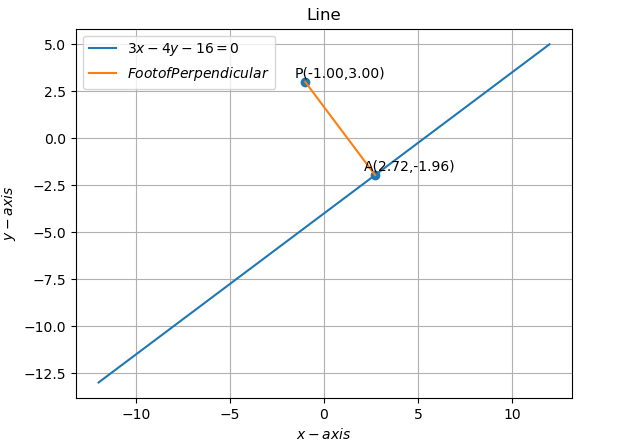
\includegraphics[width=\columnwidth]{chapters/11/10/3/14/figs/lines.png}
	\end{center}
\caption{}
\label{fig:chapters/11/10/3/14/Fig}
\end{figure}
